\documentclass{beamer}

\usepackage[utf8]{inputenc}
\usepackage[spanish]{babel}
\usepackage{beamerthemeshadow}
\usepackage{times} %font times
\usepackage[T1]{fontenc} %% Usar la codificaci�n T1
%\usepackage{apacite}
%\usepackage{fontspec}
%\usepackage[latin1]{inputenc}
\usepackage{multicol}
\usepackage[numberedbib]{apacite}

%para que cuando se seleccione un texto las letras acentuadad y las � se copien bien
\usepackage{enumerate}
\usefonttheme{professionalfonts}

\newtheorem{defi}{Definición} 



\mode<presentation>{
\usetheme{Frankfurt}
\setbeamercovered{transparent}
 \setbeamertemplate{navigation symbols}{}
 \usecolortheme{beaver}
 \setbeamercolor{local structure}{fg=darkred}
\setbeamercolor{structure}{fg=darkred}



}

\makeatletter
\defbeamertemplate*{footline}{Dan P theme}
{
  \leavevmode%
  \hbox{%
  \begin{beamercolorbox}[wd=.2\paperwidth,ht=2.25ex,dp=1ex,center]{author in head/foot}%
    \usebeamerfont{author in head/foot}URJC
  \end{beamercolorbox}%{}{~~(\insertshortinstitute)}
  \begin{beamercolorbox}[wd=.7\paperwidth,ht=2.25ex,dp=1ex,center]{title in head/foot}%
    \usebeamerfont{title in head/foot}\insertshorttitle
  \end{beamercolorbox}%
  \begin{beamercolorbox}[wd=.1\paperwidth,ht=2.25ex,dp=1ex,right]{date in head/foot}
\insertframenumber{} / \inserttotalframenumber\hspace*{2ex} 
  \end{beamercolorbox}}%
  \vskip0pt%
}
\makeatother


\title{Uso de técnicas predictivas para la planificación de grupos en Secundaria y FP}
\vspace{-5mm}
\author{Universidad Rey Juan Carlos}

\institute{\textbf {Autor: Abel de Andrés Gómez\\ Tutor: Aurelio Berges García}} % auteur
\date{{\small \today}}



\begin{document} %inicio del documento

%portada
\begin{frame}[plain]{}
\begin{center}

\includegraphics [width =0.3 \textwidth ]{figures/escudo_urjc} %logo de la U en carpeta figures
\vspace*{-5mm}

\end{center}

\titlepage
\end{frame}

%indice
\begin{frame}
\frametitle{Índice} %Esquema es el titulo de la diapositiva
\begin{multicols}{2}
	\tableofcontents
\end{multicols}
\end{frame}




%\begin{frame}[plain]<beamer>{Outline}
%\tableofcontents[currentsection,currentsubsection]
%\end{frame}

%introducci�n

\section{Introducción} % Nueva Secci�n
\subsection{Introducción} % Nueva Subsecci�n

\begin{frame}[allowframebreaks=1]
\frametitle{\secname : \subsecname}
\begin{block}{¿Que es la Sobrepoblación en el aula?}  % define un marco
Es el exceso del número de estudiantes que se encuentran en un espacio determinado cuya capacidad no es adecuada para acogerlos ni cuenta con las condiciones adecuadas para el buen desenvolvimiento de los mismos. \cite{LILIA2013}
\end{block}

\begin{block}{¿Que es la ratio?}  % define un marco
Es la relación entre el número de alumnos y profesores, es un factor importante a la hora de realizar la planificación de los recursos.
\end{block} %acaba marco
\framebreak
\begin{itemize}
	\item La ratio creció en España en 2012 un 20\%, ahorrándose así 464 millones de euros.
	\item Las ratios en España son superiores a la media de la OCDE y la UE22.
	\item Los recursos de las administraciones publicas no son infinitos.
	\item \textbf{¡Se debe planificar!}
	
	
\end{itemize}
	
\end{frame}

\subsection{Objetivos}
\begin{frame}[allowframebreaks=1]
\frametitle{\secname : \subsecname}



\begin{itemize}
	\item Seleccionar variables de interés, relativas a la resolución de la necesidad anteriormente expuesta por Unidad de Planificación, que aporten valor en el desarrollo de este TFM. 
	\item Estudiar la relación entre dichas variables con el  propósito de comprender el contexto de la sobrepoblación en el aula y la planificación de grupos.
	\item Probar distintos modelos predictivos y seleccionar aquellos que aporten mayor precisión en la predicción de los grupos. 
	\item Obtener y utilizar el modelo de mayor precisión para realizar predicciones.
	
\end{itemize}
	
\end{frame}


\section{Justificación teórica}
\begin{frame}
\frametitle{\secname : \subsecname}


\end{frame}

\section{Propuesta de intervención}
\begin{frame}
\frametitle{\secname : \subsecname}


\end{frame}

\section{Diseño de la investigación}
\begin{frame}
\frametitle{\secname : \subsecname}
\begin{figure}[htb]
\centering
\caption{Fases del ciclo de vida de CRISP-DM. Recuperado de \protect\citeA{IBMCRISP2012}.}
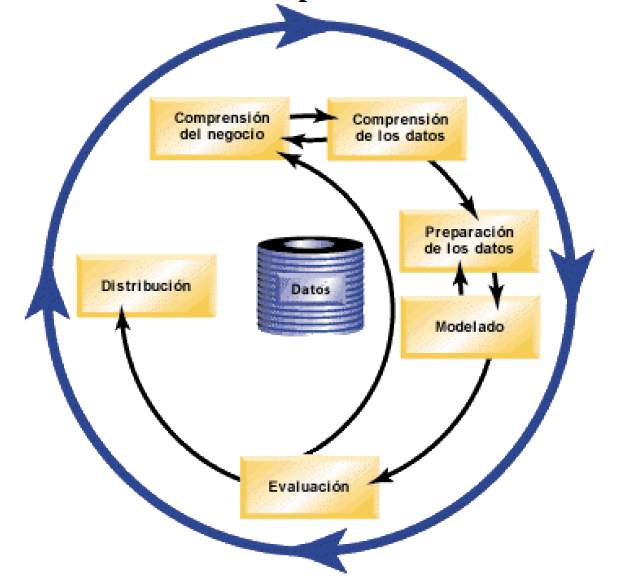
\includegraphics[width=0.6\textwidth]{../TemplateTFM/recursos/CRISPCicloIBM}
\end{figure}

\end{frame}

\section{Analisis de Resultados}

\subsection{Análisis exploratorio}
\begin{frame}
\frametitle{\secname : \subsecname}
 \begin{itemize}
 	\item La media de la ratio de la Comunidad de Madrid es de 0,88, por lo tanto los centros educativos no están sobrepoblados.
 	\item Las variables de numero de alumnos y número de grupos son importantes a la hora de predecir el numero de grupos finales.
 	\item La DAT que sufre mayor sobrepoblación en las aulas es la DAT-Centro, seguida de la DAT-Sur.
 	\item Las variables que mayor correlacionan con la \textbf{ratio} son: numero de alumnos, servicio de comedor, naturaleza del centro y código genérico del centro.
 	\item Las variables que mayor correlacionan con el\textbf{ numero de grupos a planificar} son:
 \end{itemize}
 

\end{frame}
\subsection{Análisis predictivo}
\begin{frame}
\frametitle{\secname : \subsecname}
\begin{itemize}
	\item Utilizando algoritmos se observan que las variables más importantes para realizar la predicción son: naturaleza del centro, numero de curso, número de unidades, nivel de enseñanza y ratio.
	\item El algoritmo que mejores predicciones obtiene es el Árbol de Decisión, seguido de la Regresión Lineal.
	\item Se observa que en los resultados de la predicción, de 4436 datos existentes para grupos, unicamente 52 grupos se modifican. De estos 52 grupos, 30 de ellos disminuyen en el numero de unidades y 22 aumentan. Se observa para este curso 2017/2018, que  \textbf{se reduce la población en el aula}.
\end{itemize}

\end{frame}

\section{Conclusiones}

\subsection{Aportaciones del TFM}

\begin{frame}
\frametitle{\secname : \subsecname}
 
\begin{defi}

\end{defi}

\end{frame}

\subsection{Conclusiones}

\begin{frame}
\frametitle{\secname : \subsecname}

\begin{columns}
 \begin{column}{6cm}
      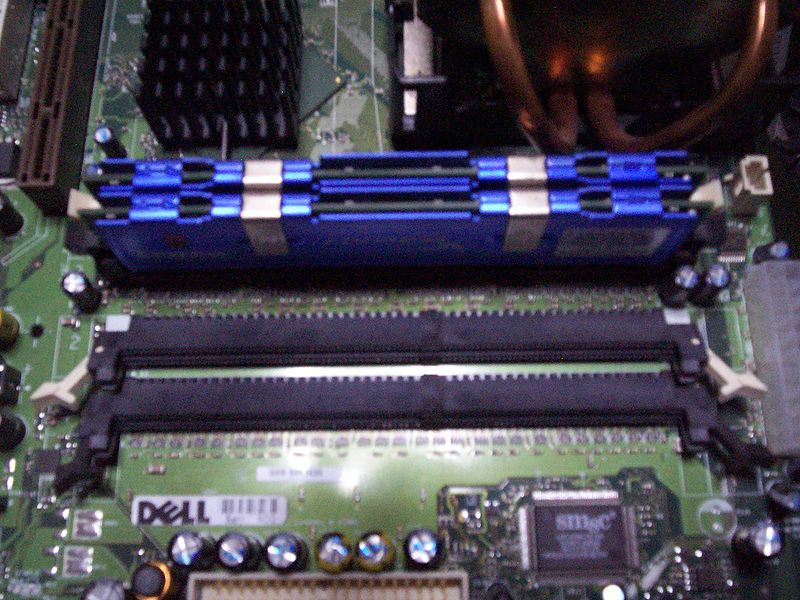
\includegraphics [width =0.8 \textwidth ]{figures/slots.jpg}
  \end{column}
  \begin{column}{6cm}
       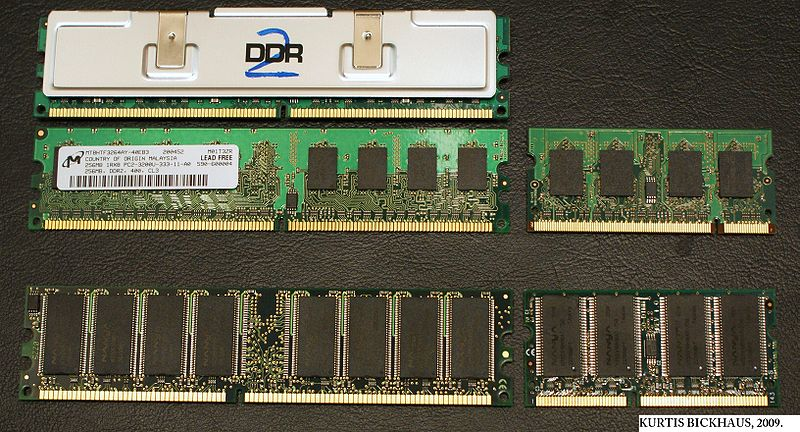
\includegraphics [width =0.8 \textwidth ]{figures/memram.jpg}
  \end{column}
\end{columns}
\end{frame}


\subsection{Lineas de Trabajo Futuro}

\begin{frame}
\frametitle{\secname : \subsecname}

\end{frame}

\begin{frame}[shrink=30]{Referencias}
\bibliographystyle{apacite} % estilo de la bibliografia
\bibliography{../TemplateTFM/referencias_prueba} % nombre del archivo .bib

\end{frame}




\end{document}


